\documentclass{article}

\usepackage{fontspec}
\usepackage{xeCJK}
\setCJKmainfont{Songti SC}
\setCJKsansfont{Heiti SC}
\setCJKmonofont{Songti SC}
\usepackage{graphicx}
\usepackage{caption}
\usepackage{subcaption}
\usepackage{booktabs}
\usepackage{listings}
\usepackage{hyperref}
\newcommand{\theHalgorithm}{\arabic{algorithm}}
\usepackage[accepted]{icml2024}
\usepackage{amsmath}
\usepackage{amssymb}
\usepackage{mathtools}
\usepackage{amsthm}
\usepackage[capitalize,noabbrev]{cleveref}
\usepackage{color}
\usepackage{colortbl}
\usepackage{float}
\usepackage[algo2e,ruled,noend,vlined,linesnumbered]{algorithm2e}
\usepackage{multirow}
\usepackage{bbding}
\usepackage{pifont}
\usepackage{wrapfig}
\usepackage{balance}

\newcommand{\cmark}{\ding{51}}
\newcommand{\xmark}{\ding{55}}
\definecolor{Gray}{gray}{0.9}
\definecolor{burntorange}{rgb}{0.8,0.33,0.0}
\DeclareMathOperator*{\argmax}{arg\,max}
\DeclareMathOperator*{\argmin}{arg\,min}
\definecolor{codegreen}{rgb}{0,0.6,0}
\definecolor{codegray}{rgb}{0.5,0.5,0.5}
\definecolor{codepurple}{rgb}{0.58,0,0.82}
\definecolor{backcolour}{rgb}{0.95,0.95,0.92}
\lstdefinestyle{mystyle}{
  backgroundcolor=\color{backcolour},
  commentstyle=\color{codegreen},
  keywordstyle=\color{magenta},
  numberstyle=\tiny\color{codegray},
  stringstyle=\color{codepurple},
  basicstyle=\tiny\ttfamily,
  breakatwhitespace=false,
  breaklines=true,
  captionpos=b,
  keepspaces=true,
  showspaces=false,
  showstringspaces=false,
  showtabs=false,
  tabsize=2
}
\lstset{style=mystyle}
\SetKwInput{KwIn}{输入}
\SetKwInput{KwOut}{输出}
\SetAlgorithmName{算法}{算法}{算法目录}
\renewcommand{\abstractname}{摘要}
\renewcommand{\figurename}{图}
\renewcommand{\tablename}{表}
\captionsetup[figure]{name=图}
\captionsetup[table]{name=表}
\makeatletter
\renewcommand{\fnum@figure}{图~\thefigure}
\renewcommand{\fnum@table}{表~\thetable}
\makeatother
\floatname{algorithm}{算法}
\renewcommand{\refname}{参考文献}
\renewenvironment{abstract}
  {\centerline{\large\bfseries 摘要}\vspace{-0.12in}\begin{quote}}
  {\par\end{quote}\vskip 0.12in}
\icmltitlerunning{AgentOptimizer}

\begin{document}
\twocolumn[
\icmltitle{以可学习函数为权重的语言模型智能体离线训练}

\icmlsetsymbol{equal}{*}
\begin{icmlauthorlist}
\icmlauthor{Shaokun Zhang}{equal,psu}
\icmlauthor{Jieyu Zhang}{equal,uw}
\icmlauthor{Jiale Liu}{psu}
\icmlauthor{Linxin Song}{usc}
\icmlauthor{Chi Wang}{msr}
\icmlauthor{Ranjay Krishna}{uw}
\icmlauthor{Qingyun Wu}{psu}
\end{icmlauthorlist}
\icmlaffiliation{psu}{宾夕法尼亚州立大学}
\icmlaffiliation{uw}{华盛顿大学}
\icmlaffiliation{usc}{南加州大学}
\icmlaffiliation{msr}{微软研究院}
\icmlcorrespondingauthor{Qingyun Wu}{qingyun.wu@psu.edu}
\icmlkeywords{机器学习，语言模型智能体，函数学习}
\vskip 0.3in
]

\chead{\small\bfseries AgentOptimizer}
\printAffiliationsAndNotice{*共同贡献}

\begin{abstract}
研究人员和实践者近来将能力强大的大语言模型（LLM）重新表述为\emph{智能体}，使其主要借助专用函数来自动完成复杂任务。
为促进 LLM 智能体的发展，我们提出一种无需修改 LLM 权重即可训练 LLM 智能体的新范式；当 LLM 难以修改或无法访问其参数时，这一范式尤其有用。
人类为了适应现实任务会不断锻造工具，而不是改变自身的生物结构去适配一组静态工具。受此启发，我们主张逐步锻造智能体的函数，使其更好地解决下游任务，而非修改 LLM 权重。
我们把函数视为可学习的“智能体参数”，并借鉴人工智能中模型训练的基本思想，开发出 AgentOptimizer：它利用 LLM 更新智能体函数，并通过回滚和早停两种策略构造一套\emph{智能体训练}算法，以简化训练过程。
大量实验表明，智能体训练范式能够显著提高代表性 LLM 智能体在多种下游任务上的性能。
我们还从学习曲线、跨域迁移能力等方面研究了智能体训练的行为。我们已将该方法集成进 \href{https://github.com/microsoft/autogen/blob/main/notebook/agentchat_agentoptimizer.ipynb}{AutoGen} 库。
\end{abstract}

\section{引言}
\label{intro}

把大语言模型（LLM）重新表述为智能体，开启了一种新的自动化范式：LLM 可以调用已有函数\footnote{文献中的“函数”有时也指工具或其他动作。}完成复杂任务~\cite{xi2023rise,wang2023survey,yao2022react,wang2023voyager,humphreys2022data,ALFWorld20}。
例如，配备“搜索维基百科”函数的 LLM 智能体可以回答知识问题；能够“发出 SQL 查询”的智能体可以检索大型数据库。
函数使 LLM 能够访问外部知识源~\cite{peng2023check}、卸载数值计算~\cite{wu2023empirical}、搜索互联网~\cite{shi2017world}，并完成更多工作~\cite{qin2023tool}。

\begin{figure}[!t]
\begin{center}
\centerline{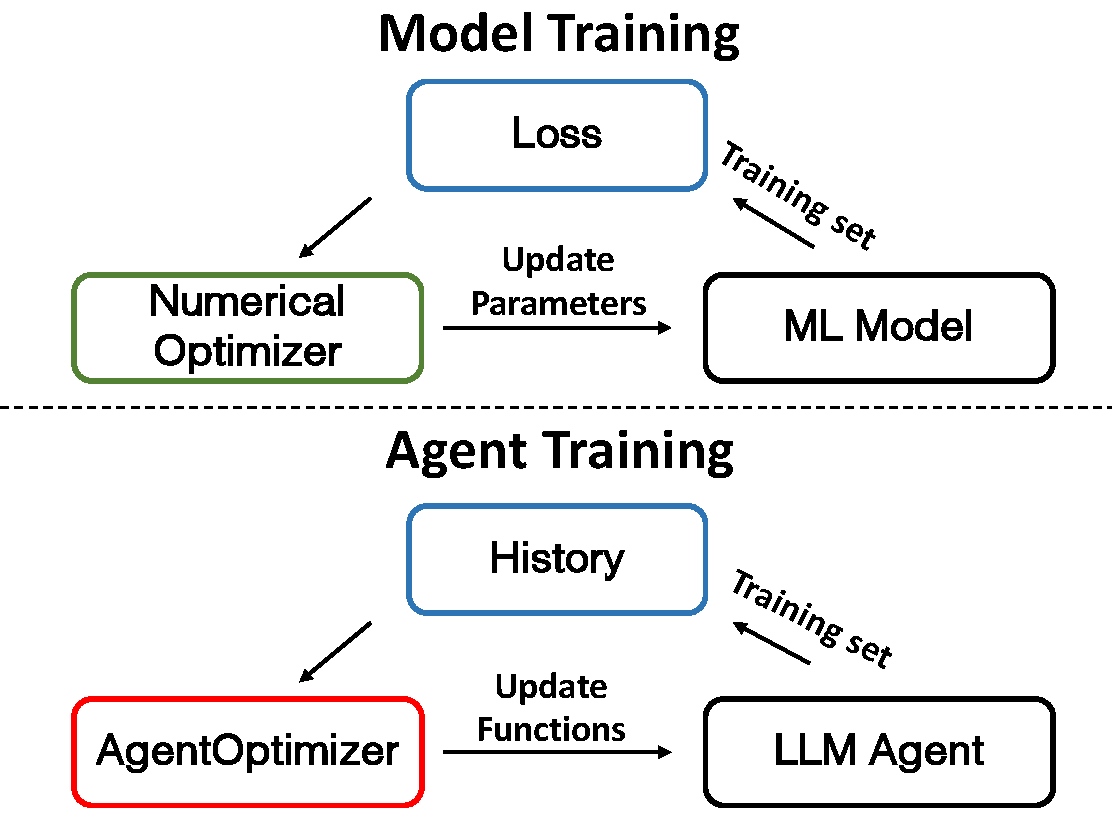
\includegraphics[width=0.8\columnwidth]{AgentOptimizer.pdf}}
\caption{模型训练与智能体训练的比较。在模型训练中，SGD、Adam 等\emph{数值优化器}~\cite{ruder2016overview}依据训练集损失优化模型权重；智能体训练则使用本文提出的 \emph{AgentOptimizer}，依据执行历史迭代更新智能体函数。}
\label{demo}
\end{center}
\vspace{-0.35in}
\end{figure}

为了让 LLM 智能体获得有用的函数，用户必须先人工创建对特定下游任务可能有帮助的函数。这一整理过程可能需要多轮迭代，因而十分耗时。
由于 LLM 是黑盒，研究者发现它们会出人意料地无法使用某些类型的函数~\cite{qin2023tool}。为此，已有研究尝试利用真实函数调用对底层 LLM 进行微调，以提升其使用既有函数的能力~\cite{qin2023toolllm,zeng2023agenttuning}。这一微调过程需要大量计算资源；更糟的是，许多 LLM 是专有模型，因而可采用的模型范围也受到限制。

人造工具会成为使用者身体能力的延伸~\cite{botvinick1998rubber}；人类会锻造工具来适应现实任务，而不是改变自身生物结构去适配静态工具。受此启发，我们提出一种新的\emph{智能体训练}范式：为 LLM 智能体“锻造”函数，使其最充分地适应训练任务。
该范式无需微调底层 LLM，并且可以从空函数集开始，因此同时解决了上述两项挑战。LLM 参数始终不变，而函数则被优化，以最大化智能体解决任务的能力。

具体而言，我们在传统模型训练与智能体训练之间建立类比（图~\ref{demo}）。第一，我们不更新模型参数，而是更新 LLM 智能体的函数，并把它们视作智能体的“可训练参数”。第二，我们不用训练集上的标量损失直接驱动更新，而是以智能体在训练任务上的执行历史和性能为依据更新函数。
由于优化发生在函数空间中，SGD、Adam 等数值优化器并不适用。为此，我们开发了 \textbf{AgentOptimizer}，让 LLM 根据当前轮次的执行历史，以及智能体生成答案与真实答案，更新智能体函数。
具体来说，AgentOptimizer 被要求通过预定义的函数操作动作（添加、修改和删除）逐步更新当前函数集，而不是在每个优化步骤重新生成整套函数。

借助 AgentOptimizer，LLM 智能体训练的总体流程如下：给定训练集和空函数集，每个轮次先在训练集上评估智能体系统，收集执行历史以及智能体生成答案与真实答案；随后把这些信息交给 AgentOptimizer，执行一次优化步骤并更新当前函数集。
为避免函数更新造成潜在性能下降，我们引入两项简单策略：回滚与早停。
若训练集性能下降，回滚会撤销当前函数更新并恢复先前状态；若连续若干次优化步骤都未提升训练集性能，早停会提前终止优化过程。

我们在三类任务上进行了广泛的实证评估：数学推理（MATH）~\cite{hendrycks2021measuring}、表格处理（TabMWP）~\cite{lu2023dynamic}和一般现实世界问题（GAIA）~\cite{mialon2023gaia}。我们使用智能体训练方法训练了两种典型系统：GPT-4+ 智能体~\cite{openai2023gpt}与 ReAct 智能体~\cite{yao2022react}。
在 MATH 数据集上，几乎所有情形下的性能都有明显提升。对于更贴近现实且更复杂的 GAIA 和 TabMWP 任务，GPT-4+ 与 ReAct 智能体经过训练后的平均性能提升分别为 6\% 和 8.5\%。
我们还通过消融实验验证智能体训练各组件的有效性，并进一步分析其扩展到大规模训练以及跨域迁移的能力。

本文贡献概括如下：
\begin{itemize}
  \item \textbf{（范式）}受机器学习模型训练基本思想启发，我们提出一套无需修改 LLM、面向给定应用构建专用 LLM 智能体的训练范式。该范式把传统模型的可学习参数类比为 LLM 智能体的操作函数，把模型损失类比为智能体在训练集上的执行历史，据此构造能够增强 LLM 智能体能力的训练机制；
  \item \textbf{（方法）}为实现这一范式，我们提出 AgentOptimizer，以替代传统模型训练使用的数值优化器。它借助 LLM 的强大能力，在 LLM 智能体的操作函数空间中工作。基于 AgentOptimizer，我们设计了带回滚和早停两项附加技术的训练算法，以简化训练流程；
  \item \textbf{（实验）}我们使用三个不同任务训练 GPT-4+ 与 ReAct 两种典型智能体系统，通过大量实验展示该范式的优势，并以消融实验和细致分析研究智能体训练的行为。
\end{itemize}

\section{方法}

下面先定义符号并说明研究问题。
我们用 $S_{\mathcal{F}}$ 表示任意带函数集 $\mathcal{F}=\{f_{1},\ldots,f_{n}\mid \forall i\in[n],f_i\in\mathcal{V}\}$ 的 LLM 智能体系统。其中，$f_i$ 表示函数空间 $\mathcal{V}$ 中可供智能体系统 $S_{\mathcal{F}}$ 使用的第 $i$ 个函数。

全文假设使用以服务形式提供的黑盒 LLM，例如 ChatGPT~\cite{openai2022gpt}。
对于任意具有训练数据 $\mathcal{D}_{train}$ 和测试数据 $\mathcal{D}_{test}$ 的任务，本文目标是找到函数集 $\mathcal{F}^{*}$，提升 LLM 智能体在未见测试数据 $\mathcal{D}_{test}$ 上的期望性能。形式化地说，
\begin{equation}
\label{eq:final_goal}
\mathcal{F}^{*}=\argmin_{\mathcal{F}\subset\mathcal{V}}E[Loss(S_{\mathcal{F}},\mathcal{D}_{test})],
\end{equation}
其中，$Loss(S_{\mathcal{F}},\mathcal{D}_{test})$ 衡量智能体 $S_{\mathcal{F}}$ 在测试数据 $\mathcal{D}_{test}$ 上的平均损失。本文的智能体训练语境下，损失定义为智能体系统解决问题失败的比例。

然而，测试集及其分布不可获得。传统机器学习模型训练通常假设训练数据与测试数据的分布相同或相近。
虽然该假设并不总成立，但在机器学习实践中，人们普遍把训练损失作为参数选择的主要指标，这是一种折中方案。

秉持相同思路，我们同样用训练数据代理测试数据，通过最小化训练数据损失，在函数空间中优化语言智能体的函数。这样便能近似估计语言智能体在未见测试数据上的表现，即
\[
\hat{\mathcal{F}}=\argmin_{\mathcal{F}\subset\mathcal{V}}Loss(S_{\mathcal{F}},\mathcal{D}_{train}),
\]
其中 $\hat{\mathcal{F}}$ 是 $\mathcal{F}^{*}$ 的近似。

\subsection{AgentOptimizer}

为得到 $\hat{\mathcal{F}}$，关键在于开发适合智能体训练的优化器：它必须能够根据智能体系统在训练集上的表现更新当前函数。
传统模型训练在数值参数空间中进行，可针对选定损失使用基于导数的优化器；智能体训练则要为智能体系统搜索最优函数集，因此现有数值模型优化器并不适用。

据此，我们提出 \textbf{AgentOptimizer}。它利用 LLM 出色的语言理解与生成能力充当优化器，迭代更新当前函数集。
具体而言，每个优化步骤都以智能体系统的当前状态、训练集执行历史和性能为提示，并要求 AgentOptimizer 更新系统函数。
直观上，这种迭代优化范式能够在巨大的语言空间中找到合适函数，类似于训练传统机器学习模型时迭代执行梯度下降。

\paragraph{AgentOptimizer 的输入。}
我们用 $H$ 表示提示 LLM 所用的信息，主要由两部分构成：第一，智能体解决训练集中每道问题时的执行历史，包括如何使用当前函数的细节；第二，在训练数据上的最终性能。
此外，输入还包括智能体系统关联的当前函数集。
这些信息使 AgentOptimizer 能够了解智能体系统的当前状态，并据此提出函数更新。

\begin{algorithm}[htb!]
\small
\captionsetup{font=small}
\SetNoFillComment
\SetAlCapNameFnt{\small}
\SetAlCapFnt{\small}
\renewcommand{\baselinestretch}{0.78}
\caption{渐进式函数更新（\texttt{AgentOptimizer.step}）}
\label{alg:2}
\KwIn{待优化函数 $\mathcal{F}^{0}$，历史信息 $H$}
\KwOut{更新后的智能体函数 $\tilde{\mathcal{F}}$}
\textbf{初始化：}$\tilde{\mathcal{F}}\gets\mathcal{F}^{0},t\gets0$
\While{$t<\texttt{MAX\_NUM}$}{
  \texttt{Action}$\gets\texttt{LLM}(\mathcal{F}^{t},H)$
  \If{\texttt{Action}=\texttt{TERMINATE}}{\texttt{break}}
  \Else{\tcp{添加、修改或删除函数}
    $\mathcal{F}^{t+1}=\texttt{Action}(\mathcal{F}^{t})$\;
    $\tilde{\mathcal{F}}\gets\mathcal{F}^{t+1}$
  }
  $t\gets t+1$
}
\textbf{返回} $\tilde{\mathcal{F}}$
\end{algorithm}

\paragraph{渐进式函数更新。}
给定输入信息 $H$，一种朴素做法是让 LLM 重新生成完整函数集，替换现有函数。
然而，这种激进的优化步骤并不明智，因为它会覆盖所有已有函数、丢弃已经建立的有用函数，并要求 LLM 一次生成多个函数。
相较之下，我们在每个优化步骤中通过预定义\emph{动作}渐进更新函数。
具体采用四种动作：1）\emph{add\_function}，添加一个可能有用的新函数；2）\emph{revise\_function}，修改一个已有函数；3）\emph{remove\_function}，删除一个已有函数；4）\emph{TERMINATE}，结束函数更新过程。
除 TERMINATE 外，所有动作都需要特定的\emph{动作参数}。例如，为执行 \emph{add\_function}，LLM 必须生成函数名称、描述、代码等动作参数，动作执行后才能把新函数加入函数集。更多细节见随官方源码保留的英文附录。
每个时间步，AgentOptimizer 都会选择一个动作，直到达到最大动作数或选择 \texttt{TERMINATE}，随后返回所得函数集。
渐进式函数更新的完整过程见算法~\ref{alg:2}。

\subsection{智能体训练}

有了 AgentOptimizer，下面给出完整智能体训练流程。
实践中，AgentOptimizer 建议的函数更新可能造成性能下降，因为 LLM 并不是更新函数的预言机。
因此，我们为训练流程提出两项简单策略来避免性能退化。

\paragraph{回滚。}
为避免函数更新后性能下降，我们采用简单而有效的回滚策略。具体而言，在每个优化步骤中，如果最新函数更新使训练集性能降低，AgentOptimizer 就撤销该更新。
此外，考虑到 LLM 已被证明能够从上下文示例中识别模式~\cite{wei2022chain}，我们还把失败的更新函数及其对应性能记录在列表中（算法~\ref{alg:1}第 11 行）。该列表将作为 AgentOptimizer 下一次生成函数时的提示。
我们预期 LLM 可利用历史失败信息生成更好的函数。一旦性能提升，列表即被清空。

\paragraph{早停。}
在极端情况下，优化过程可能陷入停滞，反复回滚却无法提高性能。
此时应当结束优化，因此我们采用早停策略：若连续 $C$ 个优化步骤都没有提升训练集性能，优化过程自动终止。

\paragraph{完整智能体训练算法。}
智能体训练伪代码见算法~\ref{alg:1}。
训练过程输入为训练数据 $\mathcal{D}_{train}$、智能体系统 $S$、最大训练轮数 $E$ 和早停阈值 $C$。
初始化步骤把初始函数列表 $\mathcal{F}_{0}$ 和初始历史信息 $H_{0}$ 设为空集。随后在每次迭代 $i$ 中，AgentOptimizer 根据历史信息 $H_i$ 优化函数列表 $\mathcal{F}_i$，得到 $\mathcal{F}_{i+1}$；再在训练集上评估更新后的函数集，为下一训练轮次取得评估信息。达到最大轮数或早停阈值时，训练过程终止。

\begin{algorithm}[!htb]
\small
\SetNoFillComment
\SetAlCapNameFnt{\small}
\SetAlCapFnt{\small}
\renewcommand{\baselinestretch}{0.78}
\caption{智能体训练}
\label{alg:1}
\KwIn{训练数据 $\mathcal{D}_{train}$，智能体系统 $S$，最大训练轮数 $E$，早停阈值 $C$}
\KwOut{增强后的智能体系统 $S_{\hat{\mathcal{F}}}$}
\textbf{初始化：}$i\gets0,r\gets0,H_0\gets\varnothing,\mathcal{F}_0\gets\varnothing$
\While{$i<E$}{
  \If{$H_i\neq\varnothing$}{$\mathcal{F}_{i+1}=\texttt{AgentOptimizer.step}(\mathcal{F}_i,H_i)$}
  \Else{$\mathcal{F}_{i+1}\gets\mathcal{F}_i$}
  $H_{i+1}=\texttt{Eval}(S_{\mathcal{F}_{i+1}},\mathcal{D}_{train})$
  \If{$H_{i+1}.loss<H_i.loss$}{
    $H_i.\texttt{fail\_record}\gets\emptyset$；
    $\hat{\mathcal{F}}\gets\mathcal{F}_{i+1}$；$i\gets i+1$；$r\gets0$
  }
  \Else{
    $H_i.\texttt{failure\_record}\gets(\mathcal{F}_{i+1},H_{i+1}.loss)$；$r\gets r+1$
    \If{$r>C$}{\tcp{早停}\texttt{break}}
  }
}
\textbf{返回} $S_{\hat{\mathcal{F}}}$
\end{algorithm}

\section{实验}

我们通过实验验证所提方法的优势。
首先在第~\ref{sec_expsetup}节介绍实验设置；随后在第~\ref{section_main_result}节使用三个数据集评估智能体训练方法，以验证其有效性；最后通过后三部分的深入研究，更全面地理解智能体训练方法。

\begin{table*}[t]
\centering
\scriptsize
\setlength{\tabcolsep}{1.8pt}
\scalebox{0.76}{
\renewcommand{\arraystretch}{1.3}
\begin{tabular}{ccccccccccccccc}
\toprule[1.5pt]
\multirow{2}{*}{\textbf{数据类型}} & \multicolumn{2}{c}{预代数} & \multicolumn{2}{c}{代数} & \multicolumn{2}{c}{中级代数} & \multicolumn{2}{c}{几何} & \multicolumn{2}{c}{计数与概率} & \multicolumn{2}{c}{预备微积分} & \multicolumn{2}{c}{数论} \\ \cline{2-15}
& 训练 & 测试 & 训练 & 测试 & 训练 & 测试 & 训练 & 测试 & 训练 & 测试 & 训练 & 测试 & 训练 & 测试 \\ \hline
GPT-4+（未训练） & 60.0\% & 78.8\% & 55.0\% & \textbf{66.3\%} & 30.0\% & 30.0\% & 30.0\% & 40.0\% & 65.0\% & 72.5\% & 5.0\% & 32.5\% & 70.0\% & 56.3\% \\
\rowcolor[gray]{0.9} GPT-4+（经训练） & \textbf{65.0\%} & \textbf{82.6\%} & \textbf{65.0\%} & 65.0\% & \textbf{40.0\%} & \textbf{38.8\%} & \textbf{40.0\%} & \textbf{42.5\%} & \textbf{65.0\%} & \textbf{76.3\%} & \textbf{10.0\%} & \textbf{35.0\%} & \textbf{80.0\%} & \textbf{67.5\%} \\
ReAct（未训练） & 55.0\% & 87.5\% & 55.0\% & \textbf{83.8\%} & 25.0\% & 50.0\% & 5.0\% & 53.8\% & 45.0\% & 73.8\% & 5.0\% & 53.8\% & 75.0\% & 68.8\% \\
\rowcolor[gray]{0.9} ReAct（经训练） & \textbf{55.0\%} & \textbf{87.5\%} & \textbf{60.0\%} & 82.5\% & \textbf{35.0\%} & \textbf{51.3\%} & \textbf{15.0\%} & \textbf{58.8\%} & \textbf{50.0\%} & \textbf{78.8\%} & \textbf{10.0\%} & \textbf{62.5\%} & \textbf{75.0\%} & \textbf{72.5\%} \\
\bottomrule[1.5pt]
\end{tabular}}
\caption{GPT-4+/ReAct 智能体在 MATH 数据集上经过与未经过智能体训练时的训练/测试准确率。表中分别给出各数据类型的准确率。可以看到，在大多数情形下，智能体训练都能使两种智能体系统获得明显更好的性能。}
\label{tab:math_main}
\end{table*}

\begin{table*}[!t]
\centering
\setlength{\tabcolsep}{22pt}
\renewcommand{\arraystretch}{0.95}
\begin{tabular}{lcccc}
\toprule
\multirow{2}{*}{\textbf{方法}} & \multicolumn{2}{c}{GAIA} & \multicolumn{2}{c}{TabMWP} \\
\cmidrule(lr){2-3}\cmidrule(lr){4-5}
& 训练 & 测试 & 训练 & 测试 \\ \hline
GPT-4+ 智能体（未训练） & 10.0\% & 16.0\% & 30.0\% & 51.0\% \\
\rowcolor[gray]{0.9} GPT-4+ 智能体（经训练） & \textbf{30.0\%} & \textbf{23.0\%} & \textbf{66.7\%} & \textbf{56.0\%} \\
ReAct 智能体（未训练） & 20.0\% & 12.0\% & 63.3\% & 59.0\% \\
\rowcolor[gray]{0.9} ReAct 智能体（经训练） & \textbf{40.0\%} & \textbf{18.0\%} & \textbf{73.3\%} & \textbf{70.0\%} \\
\bottomrule
\end{tabular}
\caption{GPT-4+/ReAct 智能体在 GAIA 和 TabMWP 数据集上经过与未经过智能体训练时的训练/测试准确率。两种智能体在两个数据集上均因智能体训练而获得更高性能。}
\label{tab:gaiatab_main}
\end{table*}

\begin{table*}[!t]
\centering
\setlength{\tabcolsep}{7pt}
\renewcommand{\arraystretch}{0.95}
\begin{tabular}{cccc}
\toprule[1.5pt]
\textbf{方法} & 数论 & 中级代数 & 计数与概率 \\ \hline
无智能体训练 & 56.3\% & 30.0\% & 72.5\% \\
智能体训练（无回滚和早停） & 63.8\% & 36.3\% & 72.5\% \\
智能体训练（无渐进式函数更新） & 60.0\% & 28.8\% & 70.0\% \\
\rowcolor[gray]{0.9} 智能体训练（本文） & \textbf{67.5\%} & \textbf{38.8\%} & \textbf{76.3\%} \\
\bottomrule[1.5pt]
\end{tabular}
\caption{以 GPT-4+ 智能体训练为例，在 MATH 的三个数据类型上消融智能体训练的不同组件。}
\label{tab:abla}
\end{table*}

\subsection{实验设置}
\label{sec_expsetup}

\paragraph{评估任务与指标。}
为评估智能体训练的有效性，我们在三类不同任务上开展实验：\emph{数学推理}、\emph{表格处理}和\emph{一般现实世界任务}。
由于 OpenAI 模型成本很高，在完整数据集上评估并不现实，因此我们依照既有工作~\cite{yuan2023craft,wu2023empirical}的设置，从这些数据集中抽样用于训练和测试。训练样本数根据 LLM 的上下文限制确定。

\textbf{（1）数学推理：}
沿用与文献~\cite{yuan2023craft}相近的设置，我们使用 MATH 数据集~\cite{hendrycks2021measuring}的一个子集，评估 LLM 智能体解决数学问题的表现。
对七种数据类型中的每一种，我们随机选择 20 个训练样本和 80 个测试样本，并分别报告各类型准确率。

\textbf{（2）表格处理：}
TabMWP~\cite{lu2023dynamic}评估智能体处理表格结构化数据的能力，每个样本含一张表和一个自然语言问题。我们随机抽取 100 个测试样本和 10 个训练样本，以精确匹配准确率衡量模型性能。

\textbf{（3）一般现实世界任务：}
GAIA 数据集~\cite{mialon2023gaia}用于评估 LLM 智能体解决无歧义现实问题的能力。我们从其公开子集中随机选取 10 个问题用于训练、100 个问题用于测试，并按原论文建议报告正确率。

\paragraph{所用智能体系统。}
我们用所提方法训练两种典型 LLM 智能体系统。

\textbf{（1）GPT-4+ 智能体：}
GPT-4+ 智能体本质上是带函数调用和代码解释器的 GPT-4。GPT-4 负责作出推理决策，代码解释器则执行 GPT-4 建议的代码和函数调用。

\textbf{（2）ReAct 智能体：}
ReAct 智能体~\cite{yao2022react}交错生成推理轨迹和任务相关动作来解决任务。在评估中，我们优化 ReAct 智能体在每次推理后可能采取的动作。

对于 GPT-4+ 和 ReAct 两种智能体，我们都以 Python 作为初始函数，使其能够执行 LLM 建议的 Python 代码。

\paragraph{模型。}
对于 MATH 和 GAIA 中更具挑战性的任务，AgentOptimizer 与智能体中的 LLM 都采用 GPT-4-1106-preview。
对于较容易的 TabMWP 任务，智能体采用 GPT-3.5-turbo-1106，而 AgentOptimizer 采用 GPT-4-1106-preview。这样做是为了更清晰地呈现智能体训练带来的改进，并不会削弱实验结论。

\subsection{主要结果}
\label{section_main_result}

\paragraph{数学推理。}
我们首先评估 GPT-4+ 与 ReAct 智能体在 MATH 数据集训练/测试划分上的性能，以及智能体训练后的表现，结果见表~\ref{tab:math_main}。
在七种数据类型上，智能体训练在多数情形下（14 项中的 11 项）提高了测试性能。此外，训练性能几乎总是提高，其余情形则保持不变。
这些结果表明，智能体训练可以产生对未见测试任务有用的函数。
有趣的是，在计数与概率问题上训练 GPT-4+ 智能体时，训练性能保持不变，而测试性能从 72.5\% 提升到 76.3\%。
这说明在某些特定情况下，即使生成函数未提升训练集性能，也可能有助于未见测试数据。

\paragraph{表格处理与一般现实世界任务。}
随后，我们在 TabMWP 表格处理任务~\cite{lu2023dynamic}和 GAIA 一般现实世界任务~\cite{mialon2023gaia}上评估，结果见表~\ref{tab:gaiatab_main}。
观察显示，智能体训练同时提高了两种智能体系统的性能。由于这两个数据集比 MATH 更贴近现实且更复杂，结果表明智能体训练能够生成通用、可用的函数，提高智能体解决现实任务的能力，因而在一定程度上具备实用价值。

\subsection{消融与分析}
\label{sec_analysis}

\subsubsection{消融实验}

我们通过消融实验评估智能体训练两类组件的有效性：1）回滚与早停；2）渐进式函数更新。
为此，我们选取训练 GPT-4+ 智能体时性能提升最大的三个 MATH 数据类型：数论、中级代数、计数与概率\footnote{预代数的提升与计数与概率相同，但它与中级代数相似，因此未被选取。}。
对于第一类组件，我们移除回滚与早停并训练到最大轮数；训练性能下降时，智能体状态不会回滚。对于第二类组件，我们把渐进式函数更新替换为一步函数生成，即直接提示 AgentOptimizer 中的 GPT-4 在每个轮次生成函数。表中也给出未经智能体训练的原始 GPT-4+ 智能体性能。

如表~\ref{tab:abla}所示，移除任一组件都会使性能大幅下降。
另一项有趣观察是，不采用渐进式函数更新的智能体训练甚至比未训练的原始 GPT-4+ 智能体更差。
这证明提示 LLM 生成函数并非易事；糟糕的函数生成方法甚至会产生负面效果。因此，需要精心设计函数生成算法。

\begin{table*}[!t]
\centering
\setlength{\tabcolsep}{8pt}
\renewcommand{\arraystretch}{0.95}
\begin{tabular}{ccccc}
\toprule[1.5pt]
\textbf{方法} & MATH 训练 & MATH 测试 & TabMWP 训练 & TabMWP 测试 \\ \hline
CREATOR~\cite{qian2023creator} & N/A & 75.0\% & N/A & 30.0\% \\
CRAFT~\cite{yuan2023craft} & 50.0\% & 73.8\% & 38.0\% & 38.5\% \\
\hline
\rowcolor[gray]{0.9} GPT-4+ 智能体（经训练） & \textbf{60.0\%} & 66.25\% & \textbf{66.6\%} & \textbf{56.0\%} \\
\rowcolor[gray]{0.9} ReAct 智能体（经训练） & \textbf{60.0\%} & \textbf{77.5\%} & \textbf{73.3\%} & \textbf{70.0\%} \\
\bottomrule[1.5pt]
\end{tabular}
\caption{训练后的智能体系统与两种典型工具创建方法在 MATH 和 TabMWP 上的比较。CREATOR 不包含训练阶段，因此没有训练性能。结果表明，经本文方法训练的 GPT-4+ 与 ReAct 智能体在多数情形下优于工具创建方法。}
\label{compare_with_tools}
\end{table*}

\subsubsection{学习曲线}

\begin{figure}[!htb]
\begin{subfigure}{0.48\linewidth}
\centering
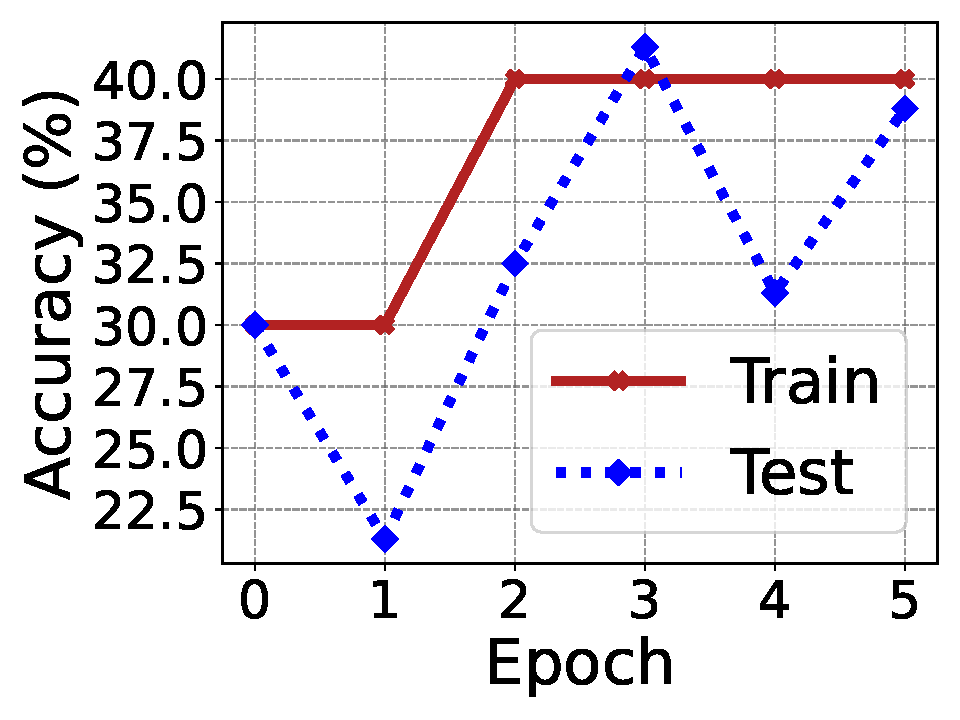
\includegraphics[width=\linewidth]{overfitting_visualizing_inte.pdf}
\caption{正例——中级代数}\label{learning_curve_a}
\end{subfigure}%
\begin{subfigure}{0.48\linewidth}
\centering
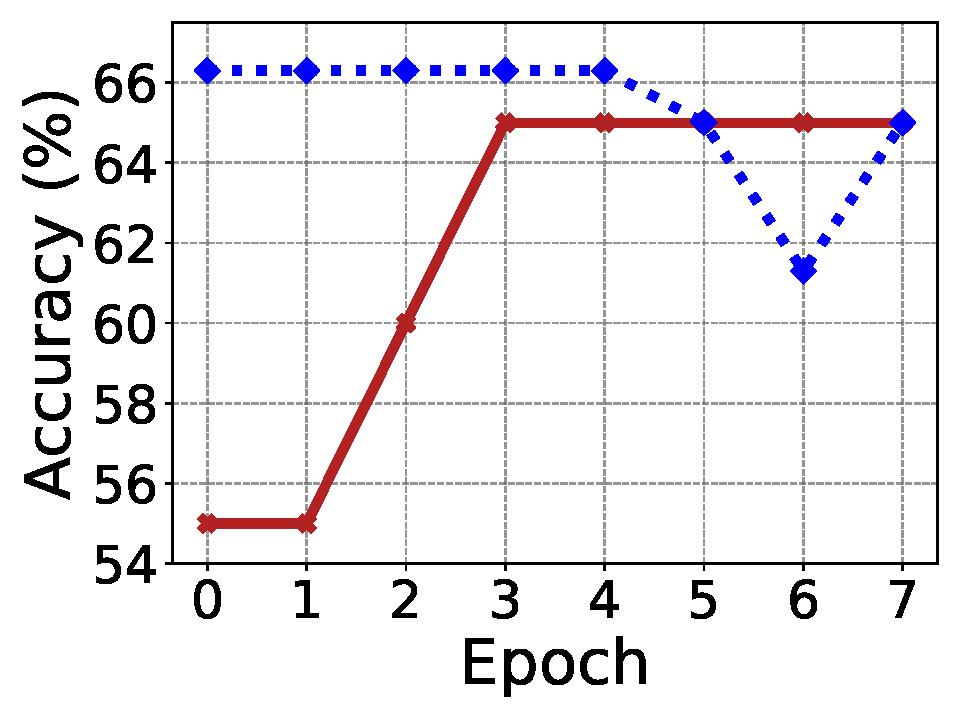
\includegraphics[width=\linewidth]{overfitting_visualizing_algebra.pdf}
\caption{负例——代数}\label{learning_curve_b}
\end{subfigure}
\caption{在 MATH 数据集上训练 GPT-4+ 智能体时，各轮次训练/测试性能的变化。为便于分析，我们选取一个训练确实提高测试性能的数据类型（正例），以及一个没有提高测试性能的数据类型（负例）。}
\label{learning_curve_ana}
\end{figure}

为便于分析，图~\ref{learning_curve_ana}展示 GPT-4+ 智能体解决数学问题时的学习曲线。
根据测试性能是否改善，把实验结果分为正例与负例：我们选择唯一未能提高测试性能的数据类型代数，以及一个与之相似但成功提高测试性能的数据类型中级代数。
对于图~\ref{learning_curve_a}中的中级代数正例，优化开始后，大多数轮次的测试性能都优于初始性能，而且测试性能总体上与训练性能正相关。这些现象为智能体训练的有效性提供了证据。
不过，最高测试性能并未出现在算法终止的最后一轮。这在一定程度上说明 GPT-4+ 智能体对训练集过拟合：训练性能不变时，测试性能却下降。
图~\ref{learning_curve_b}中的代数负例也呈现相似现象，即训练性能不变而测试性能下降。
我们还发现训练性能提高而测试性能保持不变的情形，表明生成工具有时通用性不足，虽不能带来帮助，但也不会损害任务求解性能。

\subsubsection{跨域迁移能力}

\begin{figure}[H]
\begin{center}
\centerline{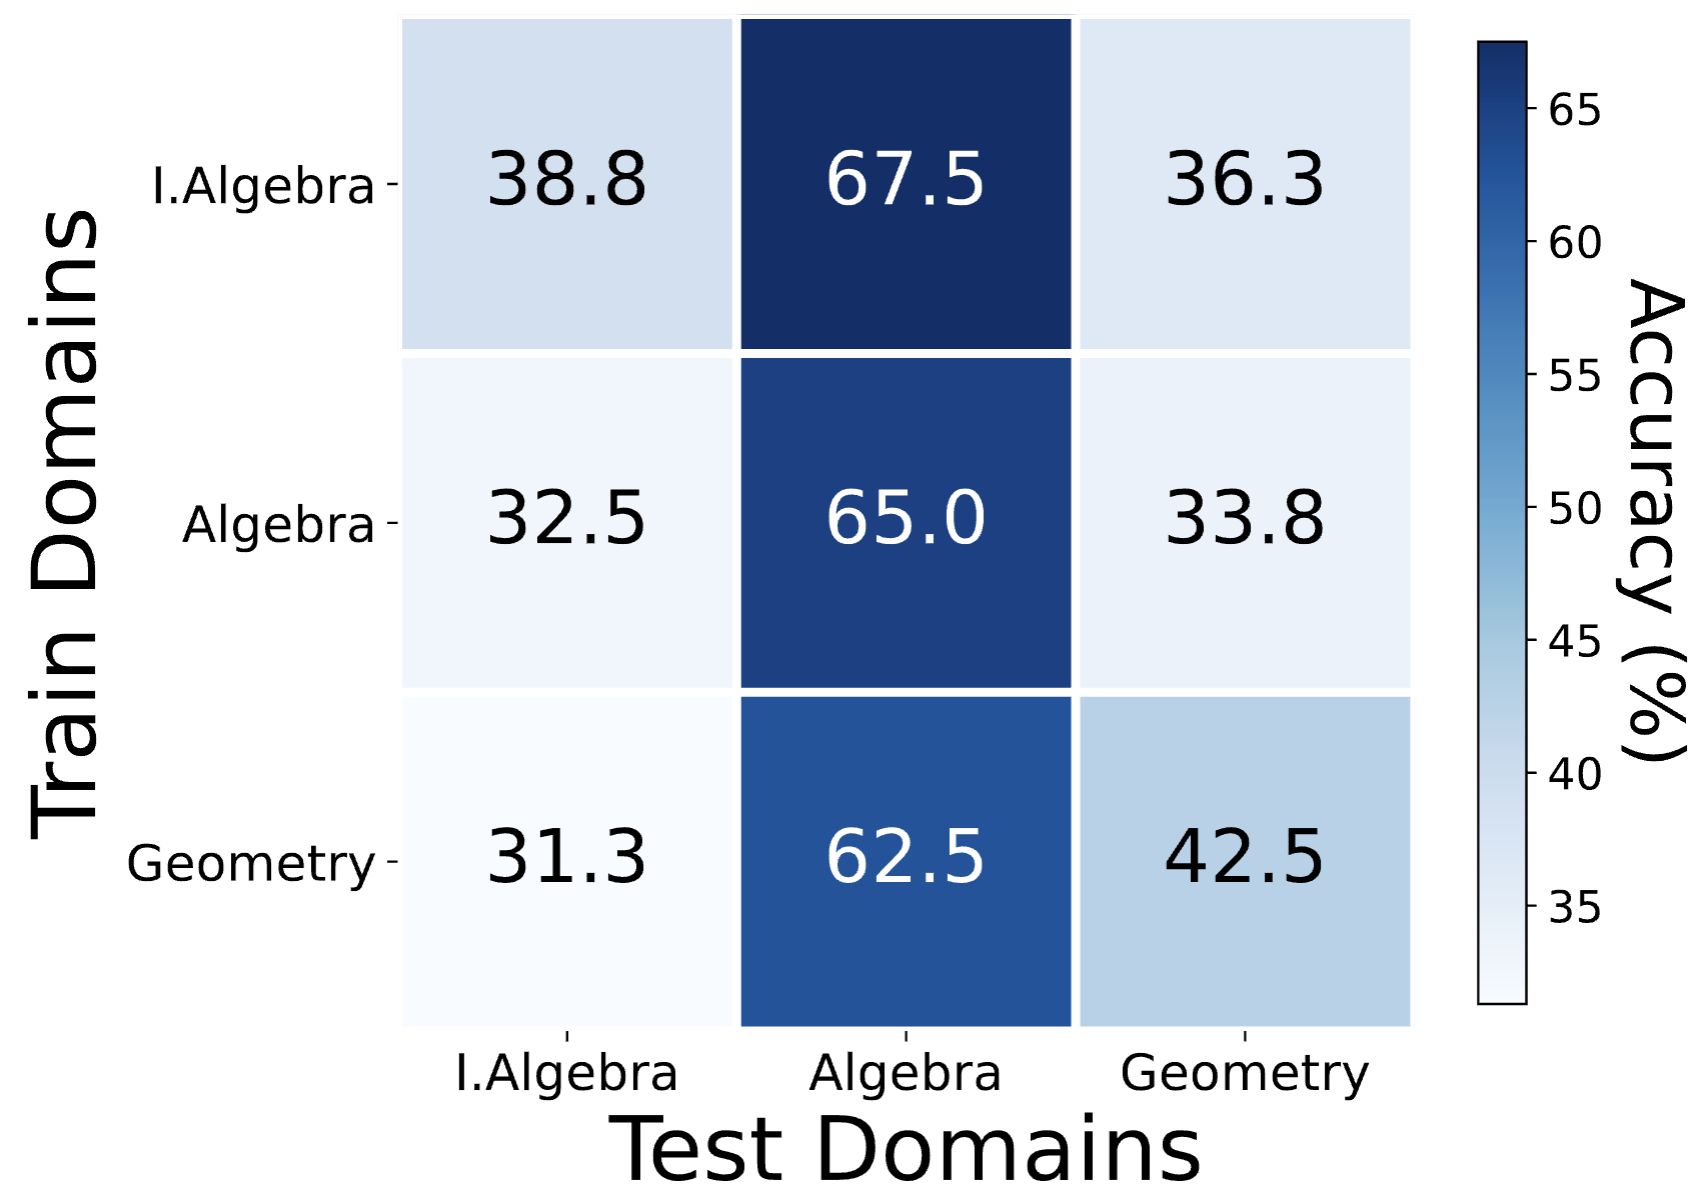
\includegraphics[width=0.59\columnwidth]{heatmap.png}}
\caption{为研究智能体训练的跨域迁移能力，图中展示在不同领域上训练后，MATH 三种数据类型的测试性能。}
\label{fig_ood}
\end{center}
\vspace{-0.35in}
\end{figure}

接下来，我们研究训练数据与测试数据并非来自同一领域时，智能体训练方法的泛化与迁移能力~\cite{zhou2022domain}。
实验使用 MATH 中的代数、中级代数和几何三种数据类型。我们有意选择两个分布相近的类型（代数和中级代数），以及一个与它们语义距离应当最大的类型（几何）。
随后，我们以不同的训练—测试配对在这三个数据集上交叉训练 GPT-4+ 智能体，并在图~\ref{fig_ood}中展示测试性能。
在多数情形下（3 项中的 2 项），当训练数据和测试数据来自同一领域时，与用其他领域训练相比，智能体训练取得最佳测试性能，这一结果符合直觉。
不过，在代数测试上出现了例外：使用中级代数训练比使用代数训练效果更好（67.5\% 对 65.0\%）。一种可能解释是，中级代数与代数分布相近，而中级代数中更困难的问题反而更便于学习适用于基础问题的基本通用函数。
另一项观察是，以几何作为训练领域时，代数和中级代数上的测试性能最差，这是因为几何的分布与另外两类都相距很远。

\subsubsection{扩展到大规模训练数据——批训练}
\label{sec:batch_train}

所提智能体训练方法存在明显瓶颈：训练数据规模受 LLM 优化器上下文长度限制，因而无法充分利用大规模训练数据。
传统模型训练也存在类似瓶颈，只不过限制来自 GPU/CPU 内存。为解决这一问题，传统机器学习采用\emph{批训练}~\cite{masters2018revisiting}，把数据集划分为较小子集（批次），在每个批次上迭代训练，从而绕开内存限制。

基于这一做法，我们为智能体训练流程提出一种直接的批训练方法。具体而言，每次训练迭代都从大规模训练数据中随机抽取一个不超过 LLM 上下文限制的训练批次，其余流程保持不变。
我们在 GPT-4+ 智能体系统上评估 MATH 的中级代数任务，训练问题为 100 个，测试问题为 80 个，测试数据与前述各节相同。
实验采用四种批大小（5、10、15、20），并分别把轮数设为 40、20、13、10，以保证用于训练的样本总数相同。最终测试性能见图~\ref{batch_abla}。
结果表明，在多数情形下，更大的训练数据并不必然提高测试性能，只有一种配置取得了轻微提升。即使批大小设为 20，与前述实验的训练数据量相同，测试性能仍下降 7.8\%。
这种下降可能源于每个轮次频繁更换训练样本，使 AgentOptimizer 无法生成稳定且有效的函数。

\begin{table*}[t]
\centering
\setlength{\tabcolsep}{13pt}
\scriptsize
\renewcommand{\arraystretch}{1.05}
\begin{tabular}{c|l}
\toprule[1.5pt]
\textbf{任务} & \textbf{最常使用的函数} \\ \midrule
\multirow{2}{*}{MATH} & evaluate\_expression, calculate\_polynomial\_roots, solve\_algebraic\_equation, calculate\_circumference \\
& calculate\_polynomial\_roots, solve\_algebraic\_equation, calculate\_complex\_magnitude \\ \midrule
GAIA & scrape\_wikipedia\_table, extract\_pdf\_text, perform\_web\_search, fetch\_web\_content \\ \midrule
\multirow{2}{*}{TabMWP} & calculate\_total\_cost, analyze\_stem\_leaf\_plot, calculate\_basic\_statistics, perform\_table\_calculation \\
& perform\_arithmetic\_operations, statistical\_analysis \\ \bottomrule[1.5pt]
\end{tabular}
\caption{为便于说明，列出 AgentOptimizer 在不同任务中生成、且在测试期间频繁使用的函数。}
\label{tab_gen_tool}
\end{table*}

\begin{figure}[!t]
\begin{center}
\centerline{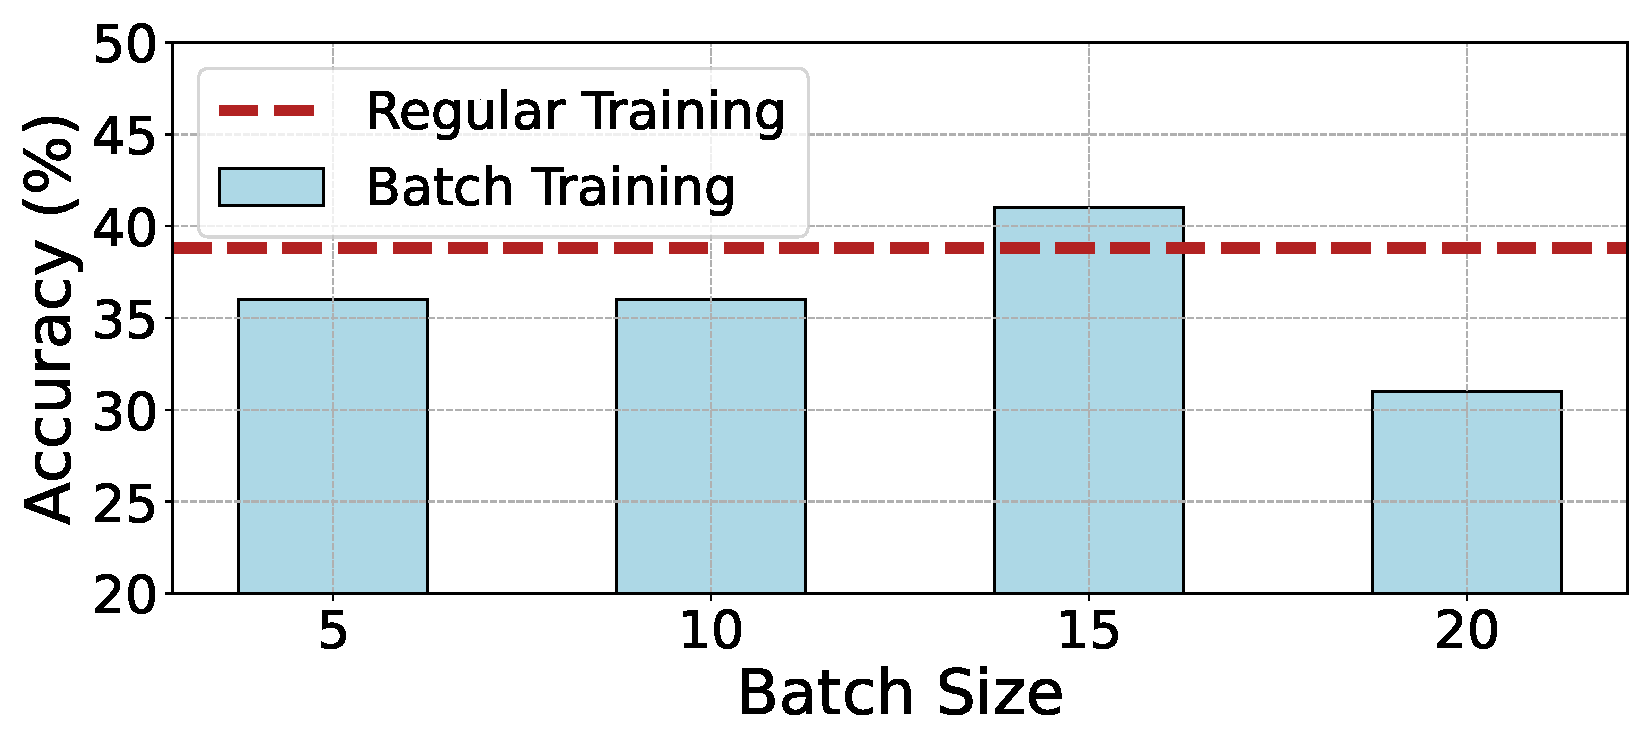
\includegraphics[width=0.7\columnwidth]{abla_batch_train.pdf}}
\caption{本文方法的“常规训练”与扩展“批训练”的比较。采用更大训练集的批训练并不必然在不同批大小设置下取得更好性能。}
\label{batch_abla}
\end{center}
\vspace{-0.35in}
\end{figure}

\subsection{智能体训练与工具创建的比较}
\label{Sec:tool}

工具创建算法~\cite{cai2023large,qian2023creator}通过提示 LLM 创建面向特定任务的工具。
由于工具创建是一次性过程，之后不会根据训练性能继续优化，其设计理念强调所创建工具“能够使用”（不会报错），而非“使用有效”（提高性能）。

本节在 MATH 和 TabMWP 数据集上，把训练后的 GPT-4+/ReAct 智能体与两种最新工具创建方法 CREATOR~\cite{qian2023creator}和 CRAFT~\cite{yuan2023craft}进行比较。
TabMWP 沿用第~\ref{section_main_result}节的实验设置。选择这两个数据集是因为相应基线代码可用，能够进行严谨比较。
为覆盖 MATH 的全部数据类型，我们从所有类型中随机抽取 20 个样本用于训练、80 个样本用于测试。
如表~\ref{compare_with_tools}所示，智能体训练后，GPT-4+ 与 ReAct 智能体的表现都优于工具创建方法，说明智能体训练是从先进大语言模型中蒸馏函数/工具的一种有前景范式。

\subsection{学习所得函数的分析}

我们对生成函数进行了深入分析。首先，表~\ref{tab_gen_tool}列出各数据集上频繁使用的函数；随后，表~\ref{tab_tool_analysis}给出模型训练第 2 轮和最后一轮成功函数调用的数量（两轮中的函数可能不同）。
我们还报告生成函数广泛采用的圈复杂度~\cite{mccabe1994software}。复杂度使用 Lizard Python 库计算；对于 GPT-4+ 和 ReAct 两种智能体的优化，表中给出每个任务工具的平均复杂度。

观察显示，多数数据集中成功函数调用数明显增加，说明与初始列表相比，优化后的函数越来越有效。
就函数复杂度而言，良好函数的复杂度应不超过 10；复杂度较低的函数较不容易触发缺陷。
三个任务上创建函数的复杂度都相对较低，说明这些函数较为可靠。

\begin{table}[!t]
\centering
\setlength{\tabcolsep}{7pt}
\renewcommand{\arraystretch}{0.9}
\begin{tabular}{cccc}
\toprule[1.5pt]
指标 & MATH & GAIA & TabMWP \\ \hline
第 2 轮 & 11 & 8 & 19 \\
最后一轮 & \textbf{23} & \textbf{10} & \textbf{41} \\
平均复杂度 & 1.2 & 3.7 & 5.0 \\ \bottomrule[1.5pt]
\end{tabular}
\caption{智能体训练第 2 轮与最后一轮成功函数调用的数量（函数可能不同），以及最后一行所示生成函数的圈复杂度。}
\label{tab_tool_analysis}
\end{table}

\section{相关工作}

越来越多研究使用 LLM 构建能够在现实任务中推理、规划并适应新观察的自主智能体~\cite{xi2023rise,wang2023survey,hong2023metagpt,yao2022react,wu2023autogen,li2023camel,babyagi,park2023generative}。
在此类 LLM 智能体中，供 LLM 与环境交互或解决子任务的函数、工具和动作发挥关键作用，但通常由人工创建~\cite{yao2022react}。
近期工作开始探索自动工具创建~\cite{cai2023large,qian2023creator,yuan2023craft}。
具体来说，Tool-maker~\cite{cai2023large}通过三个示例创建工具，再用三个验证样本检验所得工具；CREATOR~\cite{qian2023creator}为每个查询创建专属工具；CRAFT~\cite{yuan2023craft}先针对特定问题创建可定制工具，再在用户查询推理时检索相关工具。
本文提出一种概念框架，把函数视作传统 AI 模型中的可学习参数，并开发通用智能体训练范式，在多个轮次中迭代改进函数。
不同于既有工作，AgentOptimizer 根据 LLM 智能体在整个训练集上的执行历史更新函数集，而不是依据单个问答对创建函数。这样不仅在函数创建时考虑特定 LLM 智能体的行为（而不是只看问答对），也更倾向于生成适用于整个训练集的通用函数。
通过把过程表述为迭代优化，AgentOptimizer 能够以试错方式，持续依据每个训练轮次的执行历史更新函数。

另一类工作同样旨在提升 LLM 智能体，但选择修改底层 LLM~\cite{patil2023gorilla,qin2023toolllm,zeng2023agenttuning}。
例如，ToolLLM~\cite{qin2023toolllm}收集大量 API 来构造指令数据，微调 LLaMA~\cite{touvron2023llama}，从而得到针对所收集 API 使用能力优化的新 LLM；AgentTune~\cite{zeng2023agenttuning}提出混合指令微调策略，通过调整 LLM 参数来增强智能体能力。
与之相反，我们探索一种不修改底层 LLM 的智能体训练新范式。当 LLM 是 GPT-4 之类无法调优的在线服务，或调优和维护新 LLM 既昂贵又耗时时，这一范式尤其有用。

此外，本文利用 LLM 的出色能力构建用于训练智能体的优化器 AgentOptimizer，模仿模型训练中的 SGD、Adam 等数值优化器。
既有工作已证明把 LLM 用作优化器是有效的~\cite{yang2023large,zhang2023using}。
不过，既有研究主要把 LLM 优化器用于提示优化~\cite{yang2023large}、超参数优化~\cite{zhang2023using}等优化问题；AgentOptimizer 则专为新型智能体训练范式设计，在每个优化步骤中通过多次添加、修改和/或删除动作渐进更新 LLM 智能体函数。

\section{结论}

本文提出一种训练专用 LLM 智能体的新方法。
核心思想是在 LLM 智能体训练与传统模型训练之间建立类比：传统模型的可学习参数对应 LLM 智能体的操作函数，模型损失函数对应智能体的历史性能指标。
借助 LLM 强大的优化能力，我们通过所提 AgentOptimizer 更新智能体函数，从而增强智能体。
我们在多个不同任务上训练两种典型智能体系统并评估所提方法，结果表明智能体训练带来了明显的性能提升。

\section*{影响声明}

本文研究旨在推动语言智能体领域发展。我们认为，这项工作具有若干需要特别指出的潜在社会影响，既包括积极影响，也包括消极影响。
积极方面，语言智能体可能成为许多现实应用的核心~\cite{hosseini2023exploratory,cai2019hello}，而本文工作可以通过增强智能体显著惠及这些应用。例如，语言智能体可作为工业机器人的核心~\cite{zeng2023large}，本文方法可能提高工作效率。
消极方面，语言智能体的发展也使增强后智能体可能被用于负面用途，例如在社交媒体上生成错误信息或有害内容~\cite{navigli2023biases}，以达到非法目的。
另一项担忧是允许语言模型改变外部环境~\cite{tian2023evil}。例如，允许语言模型在计算机中执行代码，可能导致意外后果~\cite{liu2024empirical}。

\balance
\bibliography{reference}
\bibliographystyle{icml2024}

\end{document}
